
\usetikzlibrary{decorations.text} % decorations.text for the text along path feature

\tikzset{AgentStyle/.style={red, draw=black, font = {\Large\bfseries\sffamily}}}% Style for main lablels
\tikzset{TStyle/.style={red, font = {\Large\bfseries\sffamily}}}

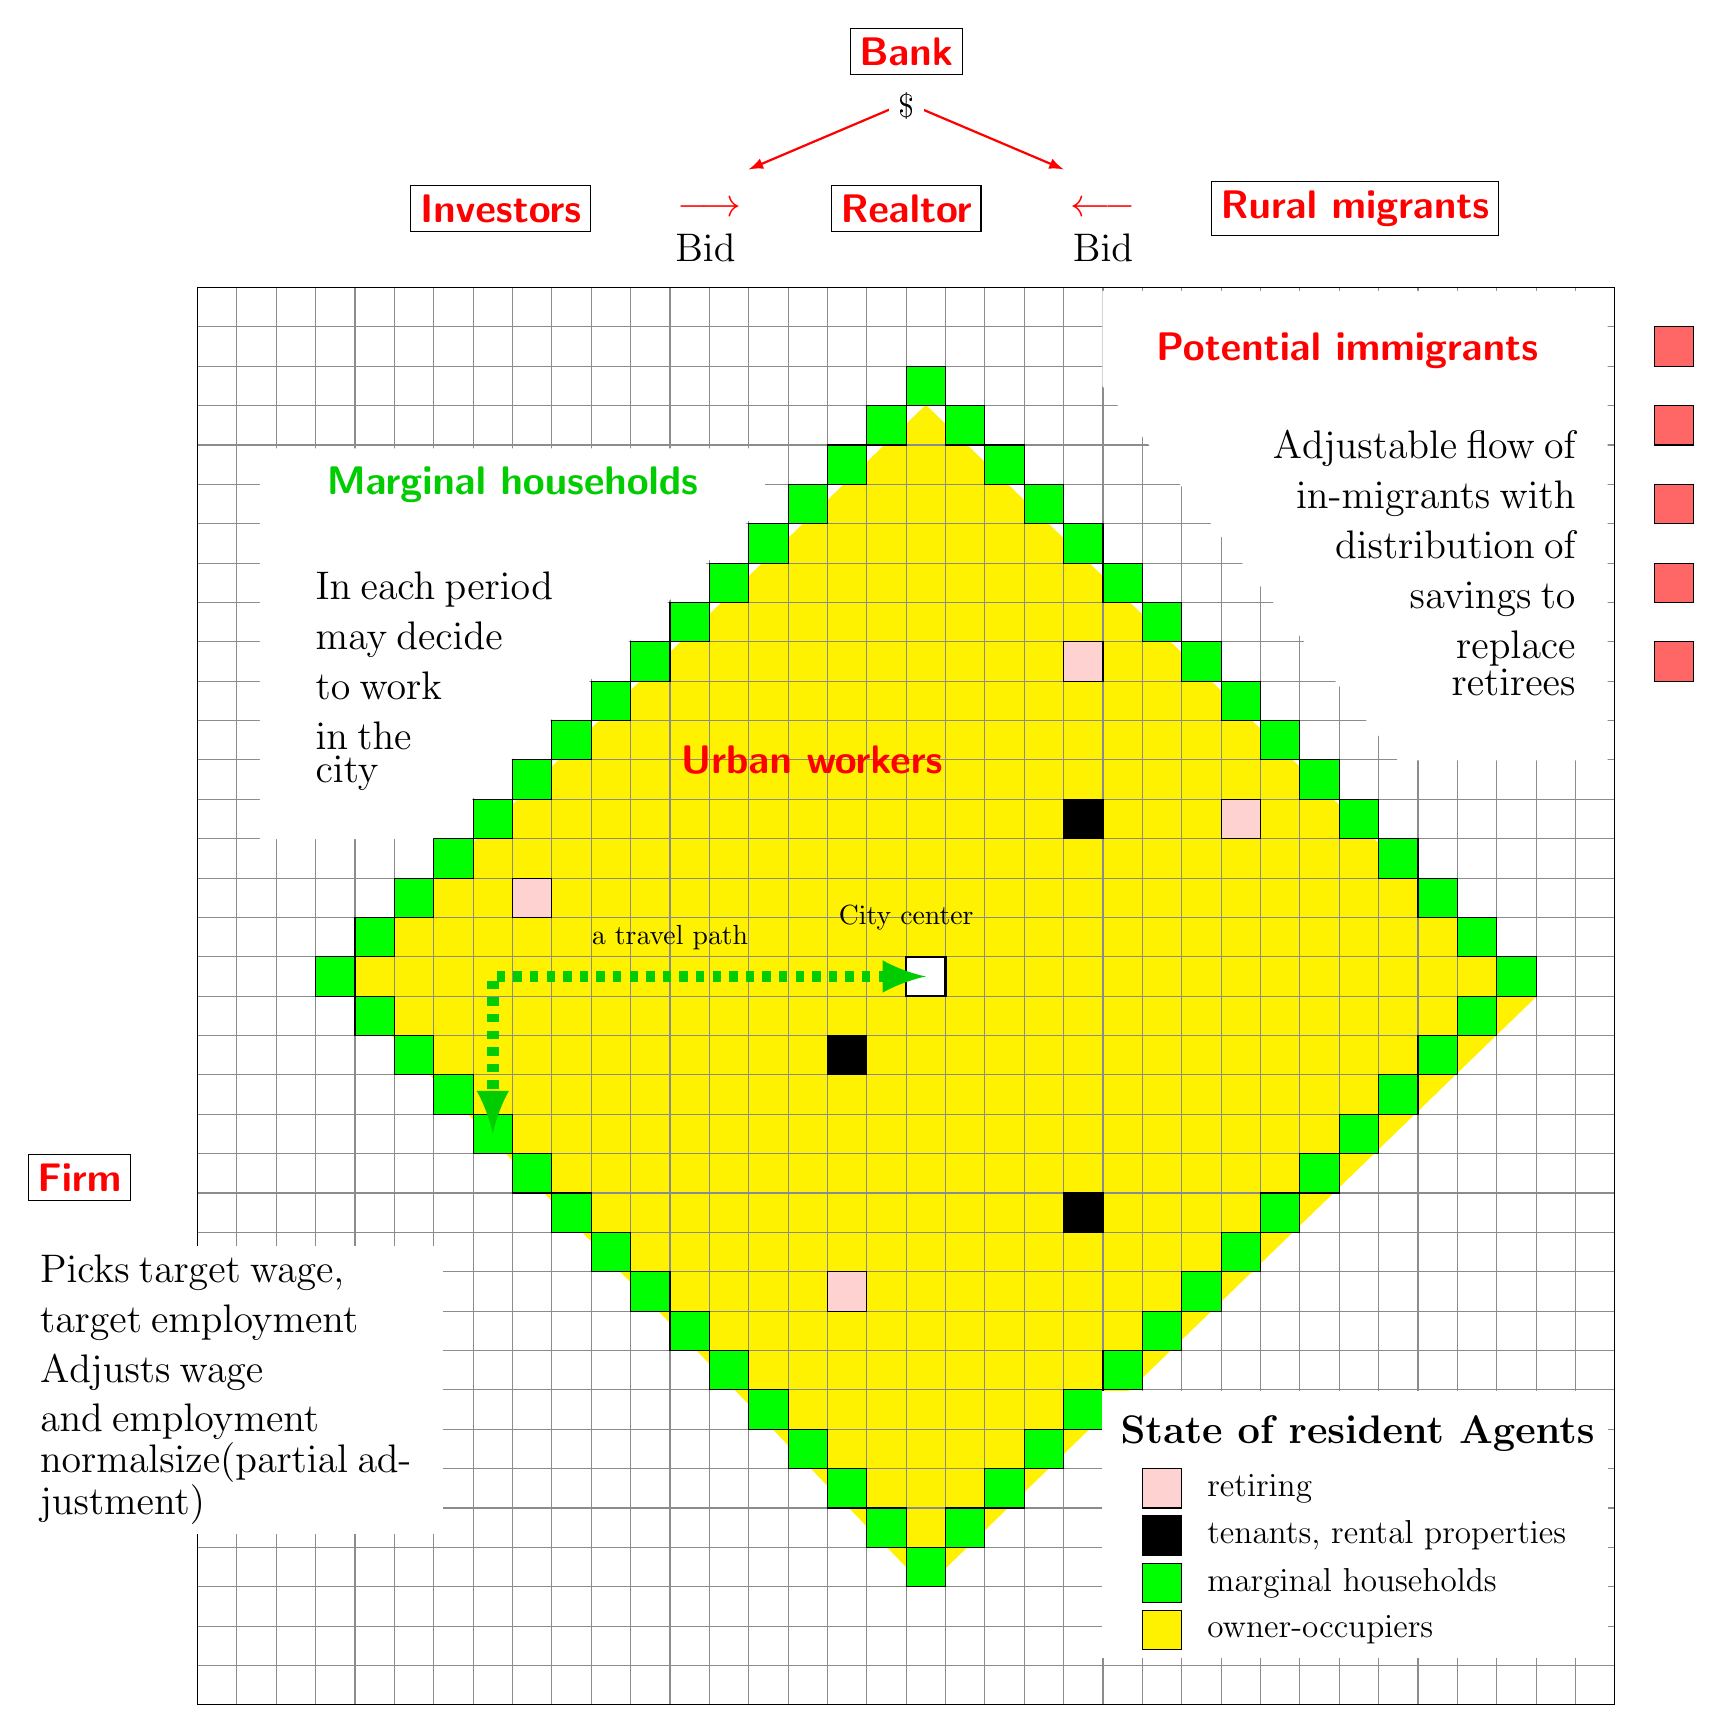
\begin{tikzpicture}
%\draw[very thin, gray!50, step=.5](-10,-10)grid(10,10);
% Locations for main label
  %Yellow square
 \draw [fill=yellow!80, yellow](8,0)--(.25,7.5)--(-7.25,.25)--(.25,-7.5)--cycle;  
 
 % grid 
  \draw[ thin, gray!90, step=.5](-9, -9)grid( 9, 9);
  \draw[  black, step=.5](-9, -9)rectangle( 9, 9);
  % center
 \draw  [fill=white, thick]  (0,0) rectangle +(.5,.5);
  \node at (0, 1) { City center};
  
% Marginal  residents _the green boundary
\foreach \z in {-7.5,-7,...,0}{ \draw  [fill=green] (\z,  {7.5+\z} ) rectangle +(.5,.5);} 
\foreach \z in {0,.5,...,7.5}{ \draw  [fill=green] (\z,  {-7.5+\z} ) rectangle +(.5,.5);}
\foreach \z in {-7.,-6.5,...,0}{ \draw  [fill=green] (\z,  {-\z-7.} ) rectangle +(.5, -.5);}  
\foreach \z in {.5,1,...,7}{ \draw  [fill=green] (\z,  {7.5-\z} ) rectangle +(.5,.5);}

% travel path
\draw [line width=1.5mm, latex-latex, dashed, black!20!green](.25, 0.25)--(-5.25,0.25)--(-5.25,-1.75);
\node at (-3,.74) {a travel path};


%.  Marginal households
\draw [fill=white, white] (-8.2, 6.95) --(-1.8,6.95)--(-1.8,6.25)-- (-6.02, 2)--(-8.2,2)--cycle;
\node at (-5,6.5)[TStyle, black!20!green!100]{Marginal households}; 
\node at (-5.5,4.)[text width=4cm] {\Large In each period \\may decide \\to work\\ in the\\ city};

%  Firm
\node [AgentStyle] at  (-10.5, -2.3){Firm};
 \node [text width=5cm, fill=white] at (-8.5, -5) {\Large Picks target wage,\\target employment\\ Adjusts wage\\ and employment \\normalsize(partial adjustment)};
 
 %Immigrants
 \draw [fill=white, white] ( 2.5,8.95) --(8.9, 8.95)--(8.9,3)-- (6.25, 3)--(2.5, 7.75)--cycle;
\node at (5.6,8.2)[TStyle]{Potential immigrants}; 
 \node [text width=6cm, , align=right] at (5.5,5.5) {\Large Adjustable flow  of \\in-migrants with distribution of\\savings to\\ replace\\ retirees };

% Locations for resident agents. (The first of these numbers is for the key.)
\def\retirees   {(2,4), (-5.,1), (-1,-4), (4,2)};			% retirees,   
\def\migrants {(9.5, 8), (9.5, 7),  (9.5,6.), (9.5,5.),   (9.5,4.)}; 	%potential migrants
\def\rental      { (2,2), (-1.,-1), (2.,-3)}; 			%rental properties

% Drawing resident agents.
\foreach \p in \retirees  {\draw [fill=pink!70] \p rectangle +(.5,.5);};
\foreach \p in \rental     {\draw [fill=black] \p rectangle +(.5,.5);};
\foreach \p in \migrants    {\draw [fill=red!60] \p rectangle +(.5,.5);};

% Labels and drawing for key for resident agents.
 \draw [fill=white, white] ( 2.5,-5.02) rectangle (8.9,-8.4);
\node at (2.6,-5.56) [right]{\textbf{\Large State of resident Agents}};  %Title for key

\node at 				(3.7,-6.25) [right]		{\large retiring};
	\draw [fill=pink!70] 	(3,-6.5) rectangle +(.5,.5);
\node at 				(3.7,-6.85) [right]		{\large tenants, rental properties};
	\draw [fill=black] 	(3,-7.1) rectangle +(.5,.5);	
\node at 				(3.7,-7.45) [right]		{\large marginal households};
	 \draw [fill=green   ] 	(3,-7.7) rectangle +(.5,.5);
\node at 				(3.7,-8.05) [right]		{\large owner-occupiers};
	\draw [fill=yellow]  	(3,-8.3 ) rectangle +(.5,.5);	 

  \node [AgentStyle] at (5.7,10){ Rural migrants};
   \node [TStyle] at (2.5,10){$\longleftarrow$};
  \node  [TStyle]  at  (-1.2,3){Urban workers};

\node at (2.5, 9.5) {\Large Bid};
\coordinate (Realtor) at (0,10);

\coordinate (Workers) at (-2,2); %Angle left 

  \node  [AgentStyle] at (0,12) {Bank};  
  \node [AgentStyle] at (Realtor) {Realtor};
  \node  [AgentStyle]  at (-5.15,10){Investors };
    \node  [TStyle]  at (-2.5,10){ $\longrightarrow$};
  \node at (-2.55, 9.5) {\Large Bid};
%  \node  [AgentStyle]  at (Workers){Investors};

  \draw [red, thick, latex-latex](-2,10.5)--(0,11.35)--(2, 10.5);
  \node [fill=white] at (0, 11.3) {\large \$};

\end{tikzpicture}
